\chapter{\acrlong{rc}}
\label{rc}

\section{Introduction}


% What is a rc
\gls{rc} is a bio-inspired artificial \gls{rnn} which is based on the \gls{esn} introduced by Herbert Jaeger in \cite{Jaeger2004}. This computation scheme is well suited for real-time data processing and for chaotic time series prediction\cite{Jaeger2004, JaegerH.2001Tesa, Lukoeviius2012}, and achieves state of the art performances in those domains, as well as in speech recognition\cite{Verstraeten2006, NIPS2010_4056, Jaeger2007}, nonlinear channel equalisation\cite{Jaeger2004} and financial forecasting \cite{financialTimeSeries}.\\

% How is it made
A \gls{rcer} is specific kind of \gls{nn}, which is a computation paradigm mimicking the behaviour of a biological brain. As can be seen on Figure \ref{nn}, the artificial neurons are merely interconnected entities carrying an activation level. As shown on Figure \ref{nn-update}, the activation level of a neuron is updated according to the connection weights of the network, also known as the synaptic matrix, and with a nonlinear function, called the \textit{activation function}, which allows \gls{nn} to perform classification tasks \cite[p.225]{bishop2006pattern}\cite[p.727]{russell2010artificial}.\\

\begin{figure}[h]
	\centering
	\begin{subfigure}{.5\textwidth}
		\centering
		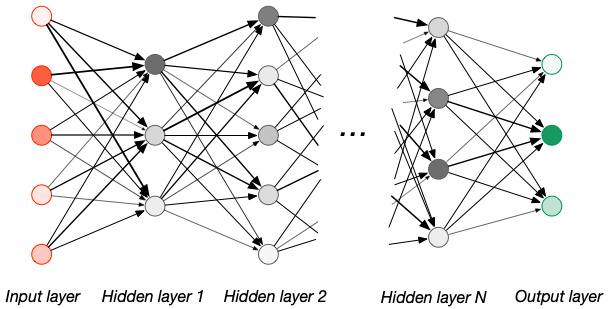
\includegraphics[height=3.5cm]{nn.png}
		\caption{High-level overview a feedforward \gls{nn} \\ \cite[p.228]{bishop2006pattern}}
		\label{nn}
	\end{subfigure}%
	\begin{subfigure}{.5\textwidth}
		\centering
		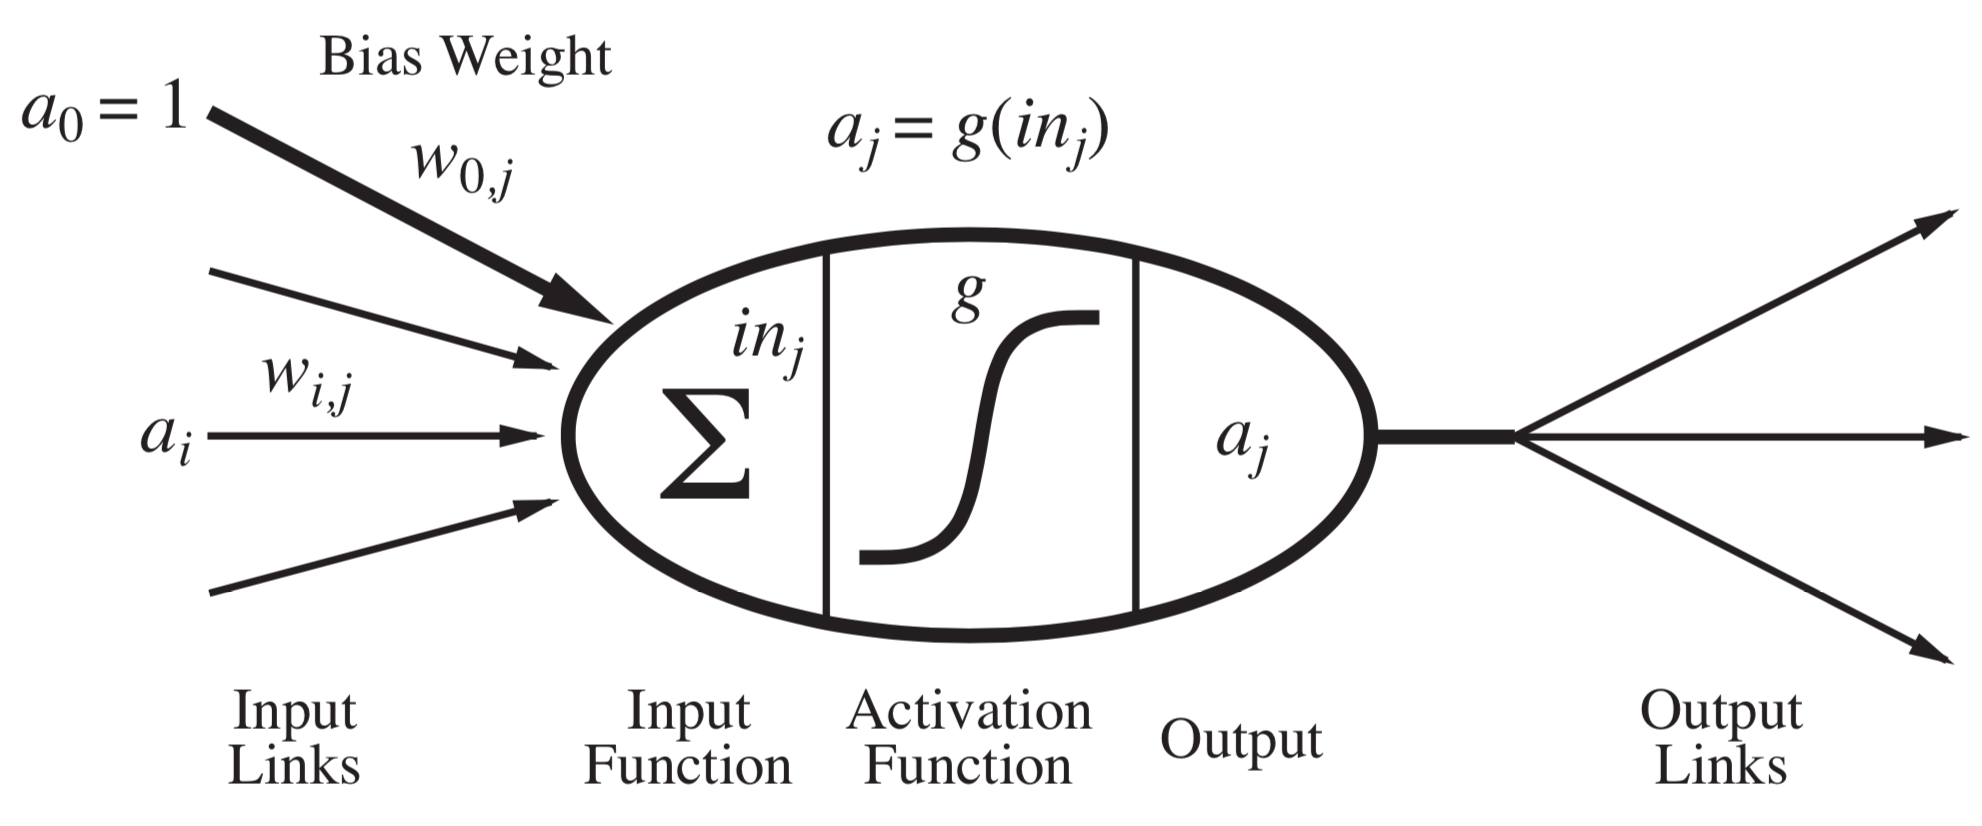
\includegraphics[height=3.5cm]{nn-update.png}
		\caption{Update of the activation level of a neuron \\ \cite[p.728]{russell2010artificial}}
		\label{nn-update}
	\end{subfigure}
	\caption{Schematic representation of a \acrlong{nn}.}
\end{figure}

% Principle of rc - changer high dimensional... par l'idée du reservoir qui sert à atteindre le esn
The activation level of the neurons making up the reservoir characterise its state, which is a time-dependent object. The neurons are interconnected in such a way that they influence the dynamic of each other, leading to a complicated evolution of the state of the reservoir. What a first glance may seem to be a mathematical nightmare turns out to be the main advantage of \gls{rc}. Indeed, by making the connection matrix as messy as possible, \textit{i.e.} by using randomness, breaking symmetries,... one notices that the effect of such a reservoir, when being fed a time-dependent signal into the input neurons, is to map it to a higher-dimensional dynamics space. \gls{rcer} reach their best performance when they are used in the echo state, which is a regime where the transients caused by the inputs are neither amplified nor damped, somehow providing a memory to the reservoir \cite{Goudarzi2014ACS}. The output of a \gls{rcer} is obtained by adequately combining the activation state of each neurons. The ideas developed in this paragraph are illustrated on Figure \ref{rc_principle}.\\

\begin{figure}[h]
	\centering
	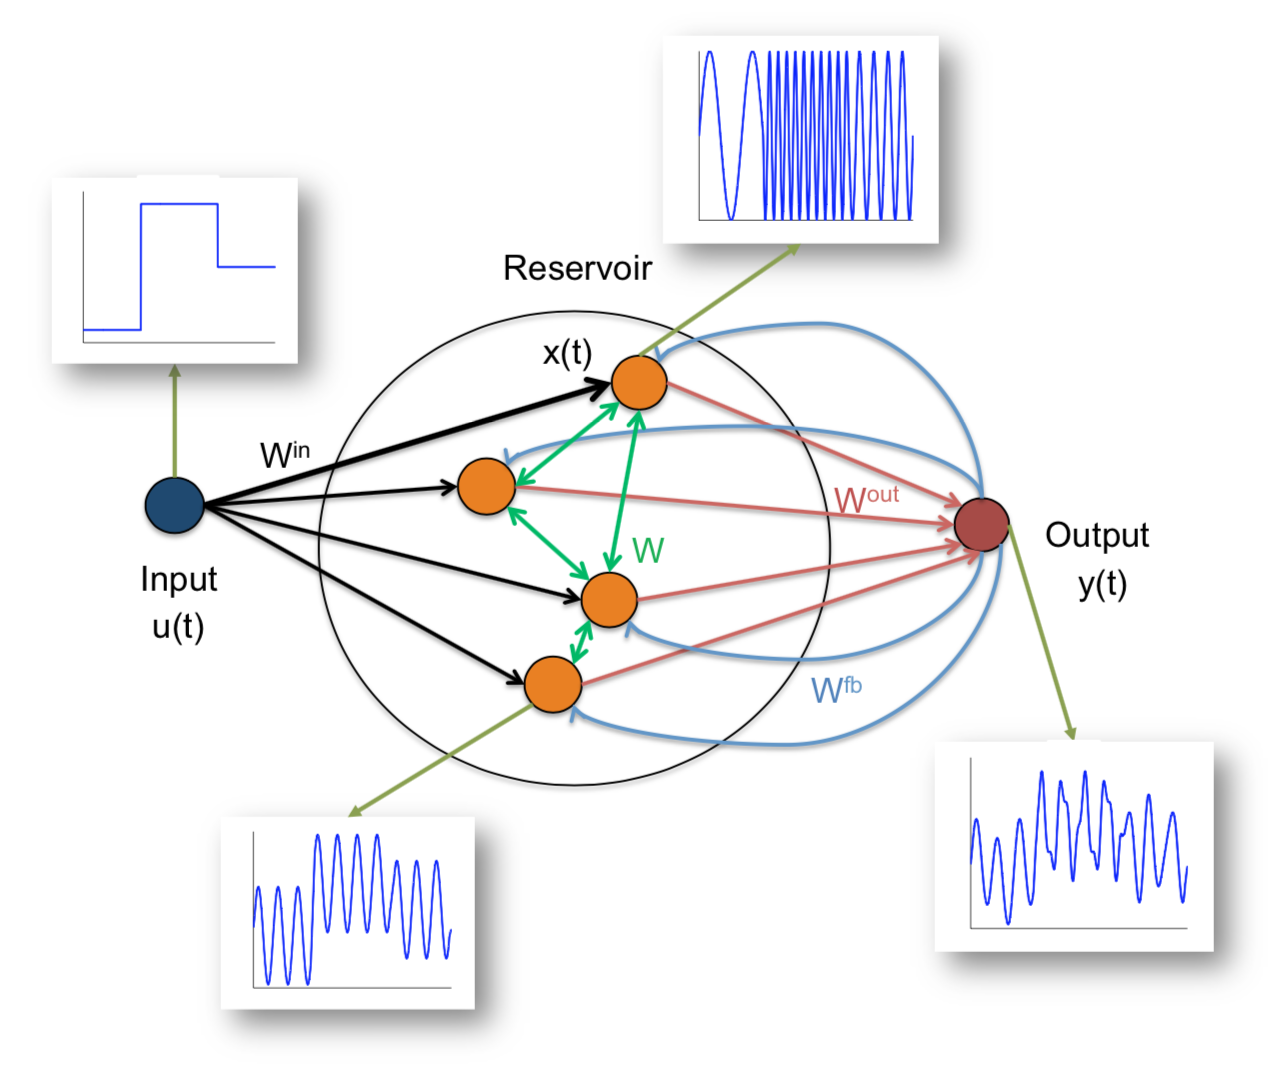
\includegraphics[width=.6\textwidth]{rc_principle.png}
	\caption{Principle scheme of a \acrlong{rcer} \cite{financialTimeSeries}}
	\label{rc_principle}
\end{figure}

% ML - different algos + sources
Regardless of the learning scheme used to train a \gls{nn}, the basic idea is always to minimise the difference between the desired and the actual outputs. In practice, this is achieved by updating the coefficients in the synaptic matrix of the \gls{nn}. On Figure \ref{nn-ml}, the learning procedure for a small portion of a feed-forward \gls{nn}, for instance the one from Figure \ref{nn}, is shown. The \gls{nn} is fed with data from the left, as can be seen with the blue arrows. The red arrows represent the error on the output being \emph{backpropagated}, which means that the learning algorithm evaluates how each connection weight of the synaptic matrix should be updated in order to decrease the output error \cite[p.241]{bishop2006pattern}. This procedure often turns out to be a really complicated task, which explains why the development of efficient \gls{ml} algorithms is such a hot topic nowadays. On the other hand, as can be seen on Figure \ref{rc-ml}, \gls{rcer} only need their output weights to be adjusted when being trained, which makes them computationally lighter. This is due to the fact the connections of the reservoir should not contain any information about the task, but should only be used to reach the \gls{esn} regime, as previously mentioned. There are two main families of training methods for \gls{rcer}. On the one hand, there is the \textit{batch learning}, which comprises the methods requiring to store a bunch of data regarding the task being taught before being able to actually compute the output weights. Once enough data is gathered, this kind of algorithms returns the optimal weights all at once. They present the advantage of involving only one training phase, after which the \gls{rcer} are ready to perform. However, the need for vast amount of data and the inability for the \gls{rcer} to adapt to an input evolving out of the range for which it has been trained are two drawbacks. On the other hand, \textit{online learning} methods allow to iteratively improve the output weights. Therefore, starting from a first guess, these algorithms will converge to workable output weights. They are much more adaptable than the batch learning ones, however, their convergence is not guaranteed and can be slow.

\begin{figure}[h]
	\centering
	\begin{subfigure}{.5\textwidth}
		\centering
		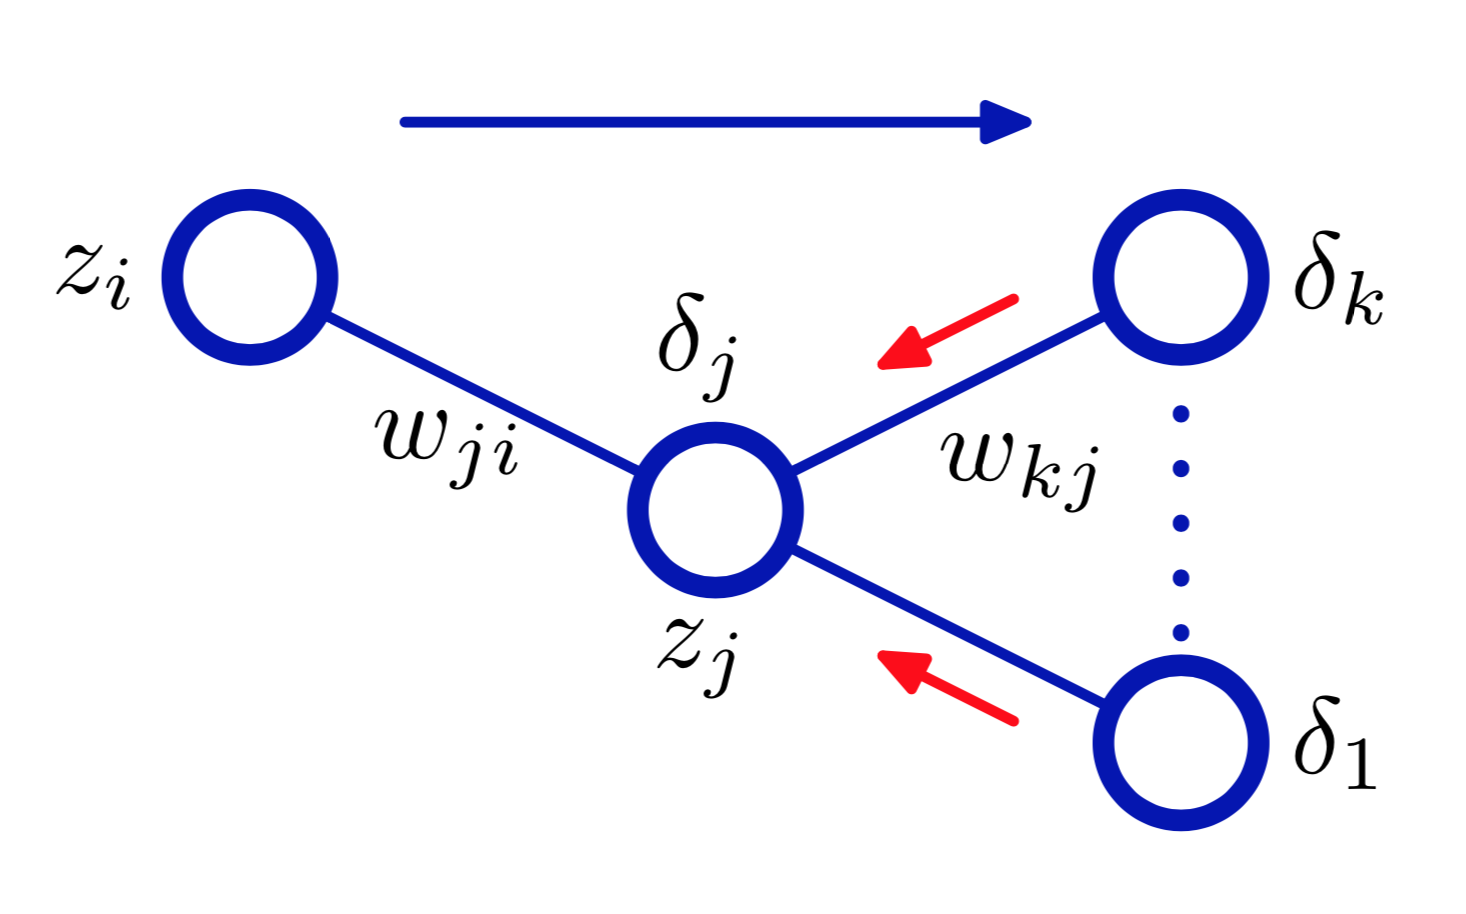
\includegraphics[height=3.5cm]{nn-ml.png}
		\caption{\acrlong{nn} \cite[p.244]{bishop2006pattern}}
		\label{nn-ml}
	\end{subfigure}%
	\begin{subfigure}{.5\textwidth}
		\centering
		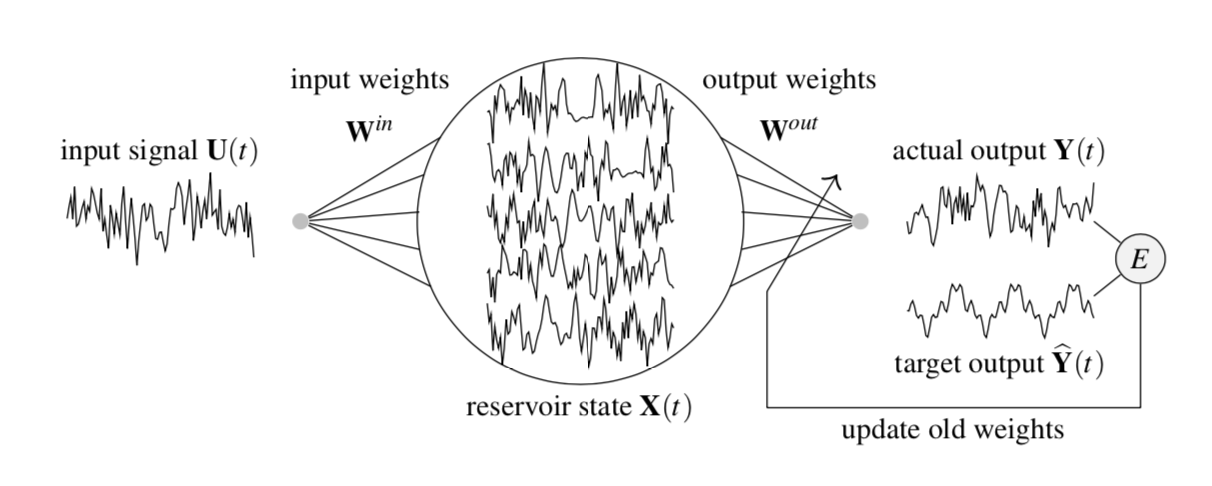
\includegraphics[height=3.5cm]{rc-ml.png}
		\caption{\acrlong{rcer} \cite{Goudarzi2014ACS}}
		\label{rc-ml}
	\end{subfigure}
	\caption{\acrlong{ml} for different kinds of \acrlongpl{nn}}
\end{figure}


